\chapter{Java 面向对象编程进阶}
\label{chp:Advanced-object-oriented-programming}

\section*{基本信息}
\sline
\begin{description}
\item[课程名称:] Java应用与开发
\item[授课教师:] 王晓东
\item[授课时间:] 第二周(根据校历,本周有两次课)
\item[参考教材:] 本课程参考教材及资料如下:
  \begin{itemize}
  \item 陈国君主编,Java程序设计基础(第5版),清华大学出版社,2015.5
  \item Bruce Eckel, Thinking in Java (3rd)
  \end{itemize}
\end{description}

\section*{教学目标}

\sline

\begin{enumerate}
\item 掌握Java包、继承、访问控制、方法重写的概念、机制和使用方法
\item 理解Java关键字super和关键字this,特别了解其指代的对象,编程中的用法
\end{enumerate}

\section*{授课方式}

\sline
\begin{description}
\item[理论课:] 多媒体教学、程序演示
\item[实验课:] 上机编程
\end{description}

\newpage
\section*{教学内容}
\sline

%%%%%%%%%%%%%%%%%%%%%%%%%%%%%%%%%%%%%%%%%%%%%%%%%%%%%%%%%%%%%%
\section{包}
为便于管理大型软件系统中数目众多的类,解决类的命名冲突问题以及进行访问
控制,Java引入包(package)机制,即将若干功能相关的类逻辑上分组打包到一
起,提供类的多重类命名空间。

\begin{figure}[htb]
\centering
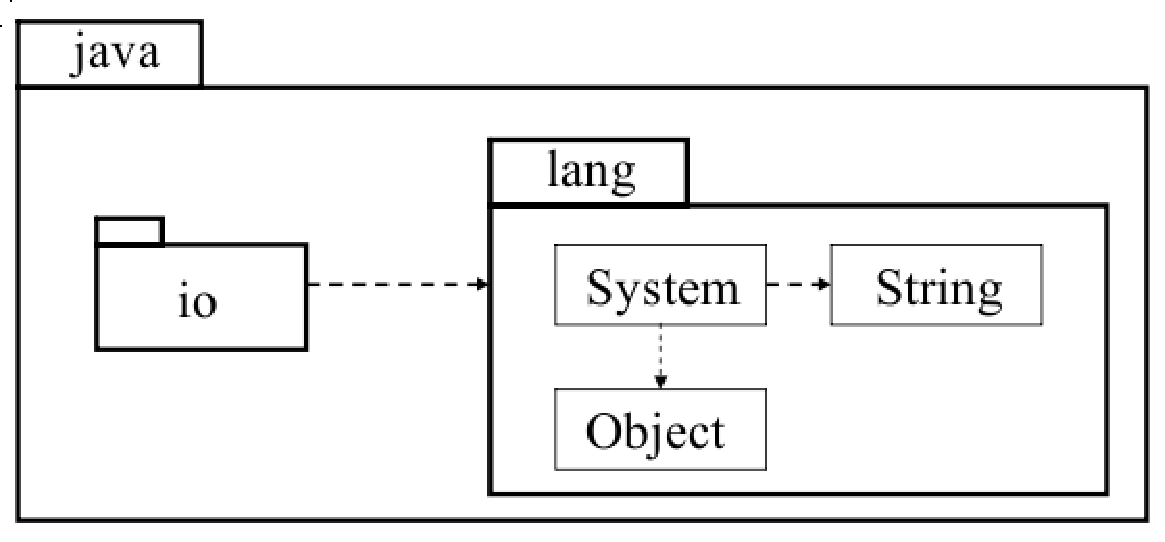
\includegraphics[width=0.6\textwidth]{images/Advanced-object-oriented-programming-1/fig-java-package.pdf}
\caption{Java包}
\label{fig:java-package}
\end{figure}

\subsection{JDK常用包}

JDK API中的常用包如表所示。

\begin{table}[!htbp]
  \centering
  \caption{JDK API常用包}
  \label{tab:java-package-list}
  \begin{tabular}{|c|c|c|}
    \hline
    {\bf 包名} & {\bf 功能说明} & {\bf 包的含义}   \\
    \hline
    java.lang & Java语言程序设计的基础类 & language的简写\\
    \hline
    java.awt & 创建图形用户界面和绘制图形图像的相关类 & 抽象窗口工具集\\
    \hline
    java.util & 集合、日期、国际化、各种实用工具 & utility的简写\\
    \hline
    java.io & 可提供数据输入/输出相关功能的类 & input/output的简写\\
    \hline
    java.net & Java网络编程的相关功能类 & 网络\\
    \hline
    java.sql & 提供数据库操作的相关功能类 & 结构化查询语言的简写\\
    \hline
  \end{tabular}
\end{table}


\subsection{包的创建}

package语句作为Java源文件的第一条语句,指明该文件中定义的类所在的包(若缺省该语句,则指定为无名包)。语法格式如下:

\begin{javaCode}
  package pkg1[.pkg2[.pkg3...]];
\end{javaCode}

\samplecode{创建包}

\begin{javaCode}
  package p1;
  public class Test {
    public void m1() {
      System.out.println("In class Test, method m1 is running!");
    }
  }
\end{javaCode}

package语句对所在源文件中定义的所有类型(包括接口、枚举、注解)均起作用。

Java编译器把包对应于文件系统的目录管理,package语句中,用“.”来指明包(目录)的层次。如果在程序Test.java中已定义了包p1,编译时采用如下方式:

\begin{shCode}
  > javac Test.java
\end{shCode}

则编译器会在当前目录下生成Test.class文件。

若在命令行下使用如下命令:

\begin{shCode}
  > java -d /home/xiaodong/work01 Test.java
\end{shCode}

“-d /home/xiaodong/work01”是传给Java编译器的参数,用于指定此次编译生成的.class文件保存到
该指定路径下,并且如果源文件中有package语句,则编译时会自动在目标路径下创建与包同名的目
录p1,再将生成的Test.class文件保存到该目录下。

\subsection{导入包中的类}

为使用定义在不同包中的Java类,需用import语句来引入所需要的类。语法格式:

\begin{javaCode}
  import pkg1[.pkg2...].(classname|*);  
\end{javaCode}

\samplecode{导入和使用有名包中的类}

\begin{javaCode}
  import p1.Test; //or import p1.*;
  public class TestPackage{
    public static void main(String args[]){
      Test t = new Test();
      t.m1();
    }
  }
\end{javaCode}

\subsection{Java包特性}

一个类如果未声明为public的,则只能在其所在包中被使用,其他包中的类即使
在源文件中使用import语句也无法引入它。可以不在源文件开头使用import语句
导入要使用的有名包中的类,而是在程序代码中每次用到该类时都给出其完整的
包层次,例如:

\begin{javaCode}
  public class TestPackage{ 
    public static void main(String args[]){ 
      p1.Test t = new p1.Test(); 
      t.m1(); 
    } 
  }
\end{javaCode}

%%%%%%%%%%%%%%%%%%%%%%%%%%%%%%%%%%%%%%%%%%%%%%%%%%%%%%%%%%%%%%
\section{继承}

\subsection{继承的概念}

继承(Inheritance)是面向对象编程的核心机制之一,其本质是在已有类型基础
之上进行扩充或改造,得到新的数据类型,以满足新的需要。

根据需要定义Java类描述“人”和“学生”信息,示例代码如下:

\samplecode{Class Person}
\begin{javaCode}
  public class Person {
    public String name;
    public int age;
    public Date birthDate;
    public String getInfo() {...}
  }
\end{javaCode}

\samplecode{Class Student}

\begin{javaCode}
  public class Student {
    public String name;
    public int age;
    public Date birthDate;
    public String school;
    public String getInfo() {...}
  }
\end{javaCode}

我们可以通过继承简化Student类的定义:

\samplecode{Class Student extends Person}

\begin{javaCode}
  public class Student extends Person {
    public String school;
  }
\end{javaCode}

Java类声明的语法格式如下:

\begin{javaCode}
  [< 修饰符 >] class < 类名 > [extends < 父类名 >] {
    [< 属性声明 >]
    [< 构造方法声明 >]
    [< 方法声明 >]
  }
\end{javaCode}

Object类是所有Java类的最高层父类,如果在类的声明中未使用extends关键字指明其父类,则默认父类为Object类。

Java只支持单继承,不允许多重继承。即:

\begin{itemize}
\item 一个子类只能有一个父类;
\item 一个父类可以派生出多个子类。
\end{itemize}

\begin{figure}[htb]
\centering
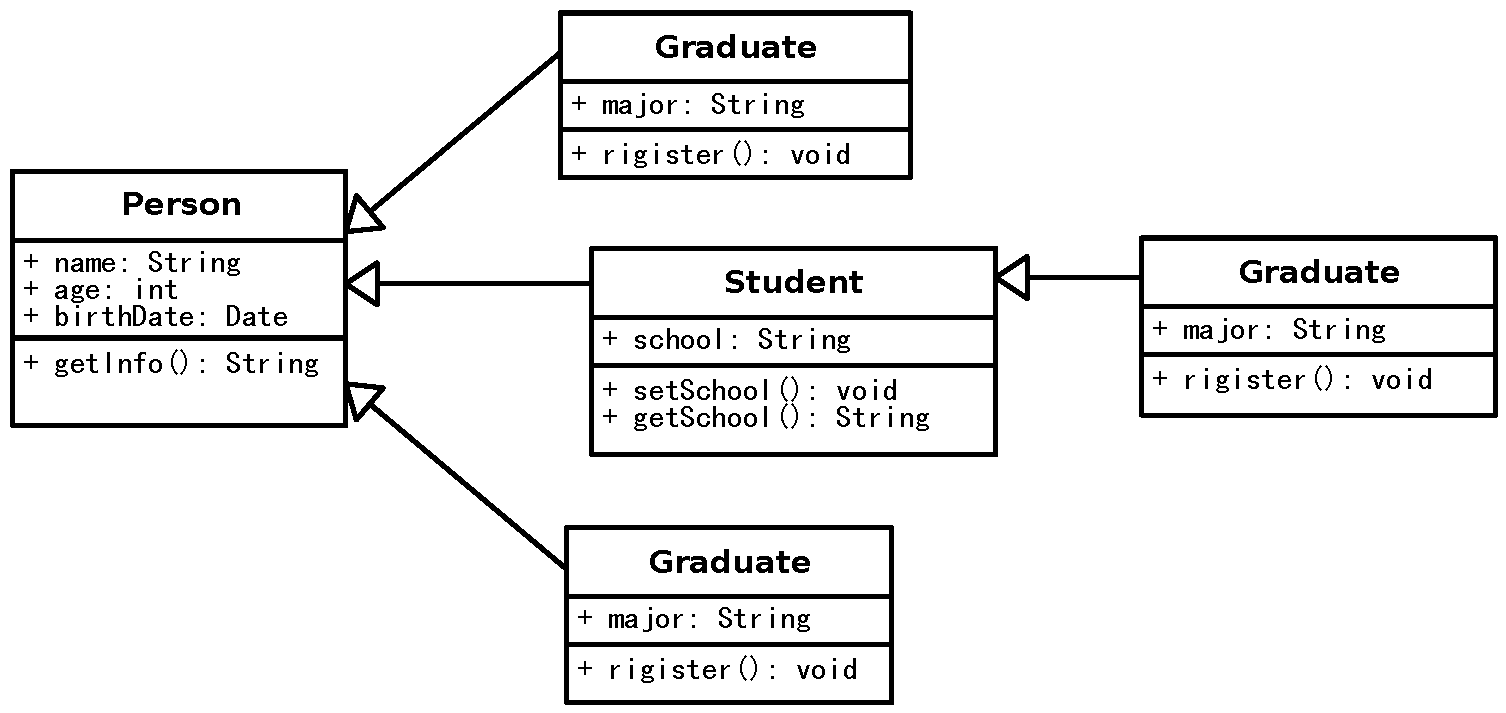
\includegraphics[width=0.9\textwidth]{images/Advanced-object-oriented-programming-1/fig-java-extends.pdf}
\caption{Java包}
\label{fig:java-package}
\end{figure}

\subsection{类之间的关系}

\begin{description}
\item[依赖关系] 一个类的方法中使用到另一个类的对象
  (uses-a)\footnote{车能够装载货物,车的装载功能(load()方法)对货物
    (goods)有依赖。}。
\item[聚合关系] 一个类的对象包含(通过属性引用)了另一个类的对象
  (has-a)\footnote{车有发动机、车轮等,Car对象是由Engine等对象构成
    的。}。
\item[泛化关系] 一般化关系(is-a),表示类之间的继承关系、类和接口之间
  的实现关系以及接口之间的继承关系。
\end{description}

\section{访问控制}

访问控制是指对Java类或类中成员的操作进行限制,即规定其在多大的范围内可以被直接访问。

\subsection{类的访问控制}

在声明Java类时可以在class关键字前使用public来修饰,也可以不使用该修饰
符。public的类可在任意场合被引入和使用,而非public的类只能在其所在包中
被使用。

\subsection{类中成员的访问控制}

\begin{table}[!htbp]
  \centering
  \caption{类成员的访问控制}
  \label{tab:java-class-member-access-control}
  \begin{tabular}{|c|c|c|c|c|}
    \hline
    {\bf 修饰符/作用范围} & {\bf 同一个类} & {\bf 同一个包} & {\bf 子类} & {\bf 任何地方} \\
    \hline
    public & yes & yes & yes & yes\\
    \hline
    protected  & yes & yes & yes & no \\
    \hline
    无修饰符 & yes & yes & no & no \\
    \hline
    private & yes & no & no & no \\
    \hline
  \end{tabular}
\end{table}

\subsection{访问控制注意的一些问题}

\begin{itemize}
\item 一般不提倡将属性声明为public的,而构造方法和需要外界直接调用的普通方法则适合声明为
  public的。
\item 在位于不同的包内,必须是子类的对象才可以直接访问其父类的protected成员,而父类自身
  的对象反而不能访问其所在类中声明的protected成员。
\item 所谓“访问控制”只是控制对Java类或类中成员的直接访问,而间接访问是不做控制的,也不该
  进行控制。
\end{itemize}

\begin{figure}[htb]
\centering
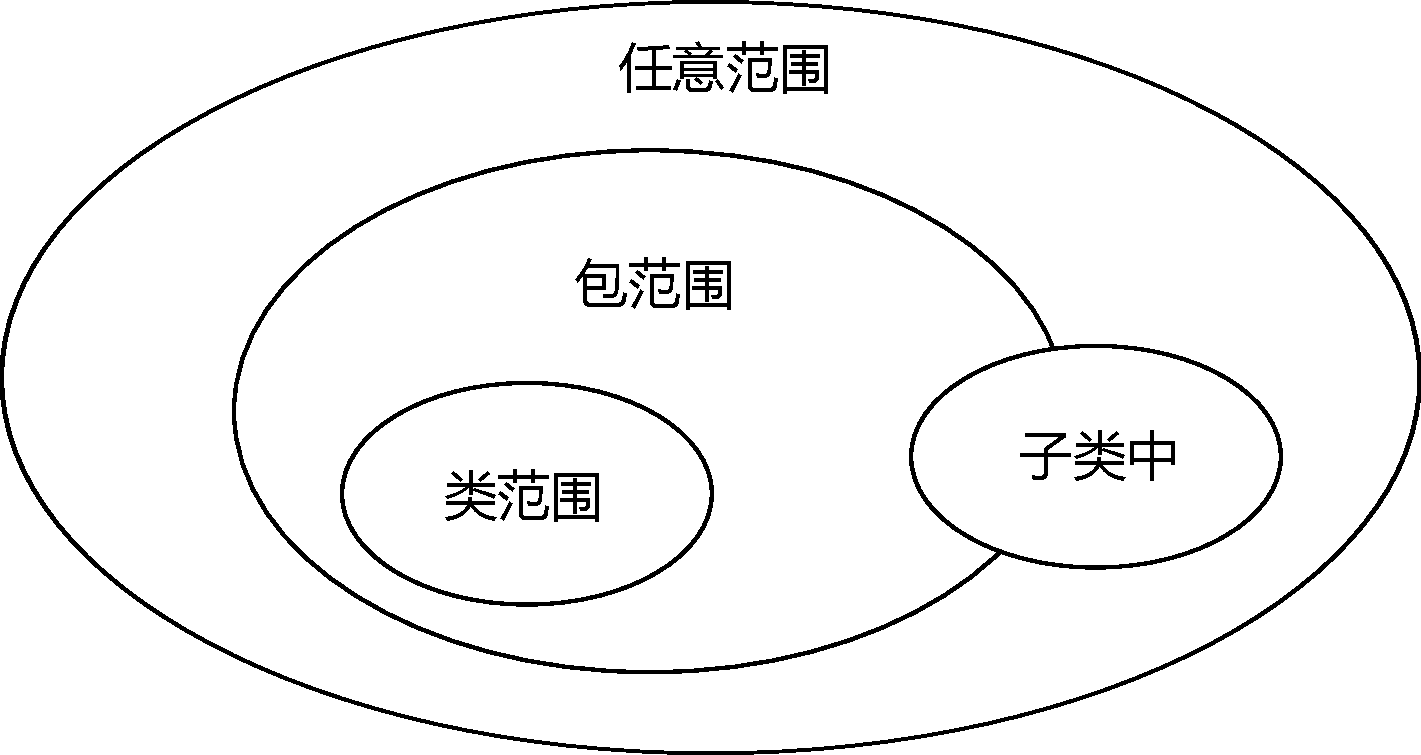
\includegraphics[width=0.6\textwidth]{images/Advanced-object-oriented-programming-1/fig-java-access-control.pdf}
\caption{Java访问控制}
\label{fig:java-access-control}
\end{figure}


\subsection{访问控制protected}

\samplecode{A.java}

\begin{javaCode}
  package p1;
  public class A {
    public int m = 5;
    protected int n = 6;
  }
\end{javaCode}

\samplecode{B.java}
\begin{javaCode}
  package p2;
  import p1.A;
  public class B extends A {
    public void mb() {
      m = m + 1;
      n = n * 2;
    }
    
    public static void main(String[] args) {
      B b = new B();
      b.m = 7;  // 合法
      b.n = 8;   // 合法
      A a = new A();
      a.m = 9 // 合法
      a.n = 10 // 非法
    }
  }
\end{javaCode}

\section{同名问题}

\subsection{方法重写}

在子类中可以根据需要对从父类中继承来的方法进行重新定义,此称方法重写(Override)或覆盖。

\begin{itemize}
\item 重写方法必须和被重写方法具有相同的方法名称、参数列表和返回值类型;
\item 重写方法不能使用比被重写方法更严格的访问权限;
\item 重写方法不允许声明抛出比被重写方法范围更大的异常类型。
\end{itemize}

\samplecode{方法重写示例:Person.java}
\begin{javaCode}
  public class Person {
    String name;
    int age;
    public String getInfo() {
      return "Name:"+ name + "\t" +"age:"+ age;
    }
  }
\end{javaCode}

\samplecode{方法重写示例:Student.java}

\begin{javaCode}
  public class Student extends Person {
    private String school;
    public void setSchool(String scholl) {
      this.school = school;
    }
    public String getSchool(){
      return school;
    }
    public String getInfo() {
      return "Name:"+ name + "\tAge:"+ age + "\tSchool:" + school;
    }
  }
\end{javaCode}

\samplecode{方法重写示例:Parent.java}
\begin{javaCode}
  public class Parent {
    public void method1() {...}
  }
\end{javaCode}

\samplecode{方法重写示例:Child.java}

\begin{javaCode}
  public class Child extends Parent {
    private void method1() {} //非法,权限更严格
  }
\end{javaCode}

\subsection{同名属性}

\begin{javaCode}
  public class Person {
    int age = 5;
    public int getAge() {
      return age;
    }
    public int getInfo() {
      return age;
    }
  }
\end{javaCode}

\begin{javaCode}
  public class Student extends Person {
    int age = 6;
    public int getAge() {
      return age;
    }
  }
\end{javaCode}

\begin{javaCode}
  public class Test {
    public static void main(String args[]) {
      Person p = new Person();
      System.out.println(p.getAge());
      Student s = new Student();
      System.out.println(s.age);
      System.out.println(s.getAge());
      System.out.println(s.getInfo());
    }
  }
\end{javaCode}

上述程序的输出结果为:

\begin{stdoutCode}
  5
  6
  6
  5
\end{stdoutCode}

\descript{对上述Student对象同名属性的几点说明}

\begin{enumerate}
\item 以“对象名.属性名”方式直接访问时,使用的是子类中添加的属性age;
\item 调用子类添加或者重写的方法时,方法中使用的是子类定义的属性age;
\item 调用父类中定义的方法时,方法中使用的是父类中的属性age,
\item 可以理解为“层次优先 就近原则”,在哪个层次中的代码,就优先使用该层次类中
  定义的属性。不提倡使用同名属性。
\end{enumerate}

\subsection{关键字super} 

在存在命名冲突(子类中存在方法重写或添加同名属性)的情况下,子类中的代码将自动使用子类中
的同名属性或重写后的方法。当然也可以在子类中{\Red 使用关键字super引用父类中的成分}:

\subsubsection{访问父类中定义的属性}

\begin{javaCode}
  super.<属性名>  
\end{javaCode}

\subsubsection{调用父类中定义的成员方法}

\begin{javaCode}
  super.<方法名>(<实参列表>)
\end{javaCode}

\subsubsection{子类构造方法中调用父类的构造方法}

\begin{javaCode}
  super(<实参列表>)  
\end{javaCode}

super的追溯不仅限于直接父类,而是先从直接父类开始查找,如果找不到则逐层
上溯,一旦在某个层次父类中找到匹配成员即停止追溯并使用该成员。

\samplecode{super用法示例A}

\begin{javaCode}
  class Animal {
    protected int i = 1;   //用于测试同名属性,无现实含义
  }

  class Person extends Animal {
    protected int i = 2;     //用于测试同名属性,无现实含义
    private String name = "Tom";
    private int age = 9;
    public String getInfo() {
      return "Name:" + name + "\tAge:" + age;
    }
    public void testI() {
      System.out.println(super.i);
      System.out.println(i);
    }
  }
\end{javaCode}

\samplecode{super用法示例B}

\begin{javaCode}
  class Student extends Person {
    private int i = 3;
    private String school = "THU";
    public String getInfo() {       //重写方法
      return super.getInfo() + "\tSchool:" + school;
    }
    public void testI() {       //重写方法
      System.out.println(super.i);
      System.out.println(i);
    }
  }
  public class Test {
    public static void main(String args[]) {
      Person p = new Person();
      System.out.println(p.getInfo());
      p.testI();
      Student s = new Student();
      System.out.println(s.getInfo());
      s.testI();
    }
  }
\end{javaCode}

上述代码的输出结果为:

\begin{stdoutCode}
  Name:Tom Age:9
  1
  2
  Name:Tom Age:9 School:THU
  2
  3  
\end{stdoutCode}

\subsection{关键字this}

在Java方法中,不但可以直接使用方法的局部变量,也可以使用调用该方法的对
象。为解决可能出现的命名冲突,Java语言引入this关键字来标明方法的当前对
象。分为两种情况:

\begin{itemize}
\item 在普通方法中,关键字this代表方法的调用者,即本次调用了该方法的对象;
\item 在构造方法中,关键字this代表该方法本次运行所创建的那个新对象。
\end{itemize}

this作为一个特殊的引用类型变量,可以通过“{\Red this.成员}”的方式访问
其引用的当前对象的属性和方法。

\samplecode{this用法示例}
\begin{javaCode}
  public class MyDate {
    private int day = 17;
    private int month = 2;

    public MyDate(int day, int month) {
      this.day = day; // A
      this.month = month;
    }
    ... // Some methods 

    public void setAll(int day, int month) {
      this.setMonth(month); // B
      this.setDay(day);
    }
  }
\end{javaCode}

\descript{关于this的归纳说明}

\begin{enumerate}
\item 在Java方法中直接给出变量名而不是“对象名.变量名”的方式访问一个变
  量,系统首先尝试作为局部变量来处理;如果方法中不存在该名字的局部变量,
  才会到方法当前对象的成员变量中查找。
\item 在Java方法中直接调用一个方法而不指定其调用者时,则默认调用者为当
  前对象this。
\end{enumerate}

\newpage
\section*{实验设计}
\sline